\chapter{Analýza}
%% Analýza a návrh implementace (včetně diskuse různých alternativ a volby implementačního prostředí).

%% V části analýzy provést rozbor jednotlivých principů + výsledky rešerší - využívat hojně informace z článků a důsledně citovat zdroje

\section{Analyzované principy objektového návrhu}

Ukázkové návrhové principy analyzované v rámci této práce jsou znázorněny na obrázku \ref{analyzed_principles}. Poznamenejme, že tzv. Demeterův zákon je speciálním případem pravidla pro \uv{low coupling}.

\begin{figure}[h!]
\centering
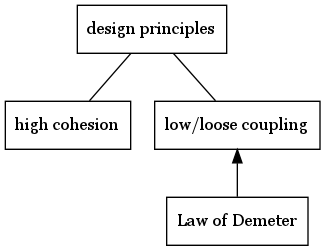
\includegraphics[width=0.5\textwidth]{./graphs/oop_design_principles.png}
\caption{Znázornění analyzovaných návrhových principů.\label{analyzed_principles}}
\end{figure}

% TODO: v rámci každého návrhového principu uvést příklad porušení
% tohoto principu (případně i příklad, který tento princip dodržuje)

% Příklad pravidla:
% ``Třídy z balíčku A nesmí záviset na jiných konkrétních třídách, ale nejvýše na rozhraních balícků B.''
%  (programování proti rozhraní namísto proti kokrétní implementaci)"

\subsection{Low coupling}

\subsection{High cohesion}

\subsection{Law of Demeter}

\section{Ukázky kódu porušujících některá z pravidel}

\subsection{Porušení principu law of Demeter}

%% TODO: use some highlighter
%% TODO: add example of demeter law violation from paper notes
\begin{verbatim}
package handlers;

public class ...

\end{verbatim}

\section{Analyzovaná doména, statický model programu v Javě}
% TODO: provide better name for this section
\subsection{Struktura Java projektu}

\subsection{Základní syntaktické elementy programovacího jazyka Java}
Grafické znázornění základních syntaktických elementů, které je převzato z \cite{Gosling:2005:JLS:1036643}, je na obrázku \ref{toplevel_elements}.
\begin{figure}[h!]
\centering
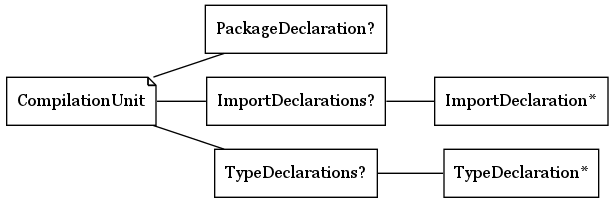
\includegraphics[width=\textwidth]{./graphs/java_top_elements.png}

\caption{Struktura základních syntaktických elementů programovacího jazyka Java.\label{toplevel_elements}}
\end{figure}
